\section{Исследовательский раздел}
\subsection{Условия исследований}
Исследование проводилось на персональном вычислительной машине со следующими характеристиками:

\begin{itemize}
\item процессор Apple M1 Pro,
\item операционная система Ventura 13.5.2,
\item 32 Гб оперативной памяти.
\end{itemize}

Временные затраты определялись с использованием библиотеки time. Затраты по памяти определялись с использованием библиотеки memory_profiler.

В данном исследовании значение параметра минимальной поддержки изменялось от значения $0.01$ до $0.5$ с шагом $0.01$. Значение минимального и максимального количества элементов было равно $2$.

\subsection{Зависимость времени исполнения от параметра минимальной поддержки}

На рисунке \ref{img:time} представлен график зависимости времени исполнения алгоритмов от заданного параметра минимальной поддержки.

\begin{figure}[H]
	\centering
	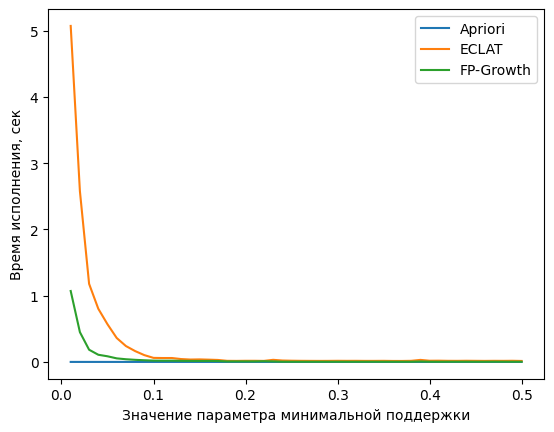
\includegraphics[width=\textwidth]{inc/time.png}
	\caption{ График зависимости времени исполнения от заданного параметра минимальной поддержки.}
	\label{img:time}
\end{figure}


\subsection{Зависимость количества занятой памяти процессом во время исполнения алгоритмов от заданного параметра минимальной поддержки}

На рисунке \ref{img:memory} представлен график зависимости количества занятой памяти процессом во время исполнения алгоритмов от заданного параметра минимальной поддержки.


\begin{figure}[H]
	\centering
	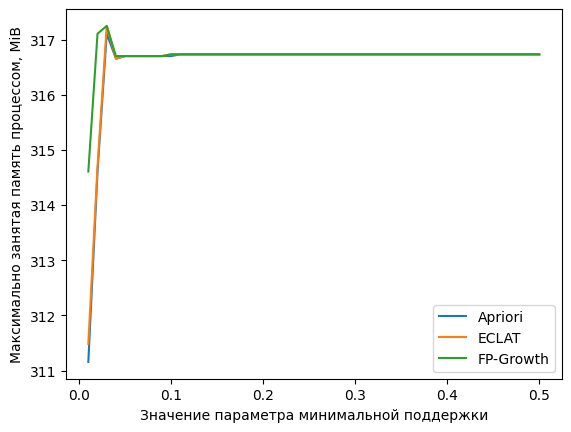
\includegraphics[width=\textwidth]{inc/memory.png}
	\caption{ График зависимости количества занятой процессом во время исполнения алгоритмов от заданного параметра минимальной поддержки.}
	\label{img:memory}
\end{figure}

\subsection*{Заключение}

В результате проведенных исследований заметно, что по времени исполнения на меньших значениях параметра минимальной поддержки самое долгое время исполнения у алгоритма ECLAT. Самым быстрым временем исполнения обладает алгоритм Apriori. В дальнейшем, при увеличении параметра, разница во времени исполнения у трех алгоритмов становится уже не такой заметной и при значении параметра минимальной поддержки равным $0.15$ уже практически отсутствует.

Также стоит отметить, что размер задействованной памяти, потребовавшейся для исполнения каждого из алгоритмов, практически одинаков. Отличия присутствуют лишь при начальных значениях величины параметра минимальной поддержки -- в данном случае однозначно можно считать, что Apriori занимает на $\approx 4$ мебибайта меньше алгоритма FP-Growth.